% IUSSP 2013 presentation
% 13_08_iussp.tex
% Begun.: 2013-08-24
% Edited: 2013-08-24

\documentclass[red]{beamer}

\mode<presentation>
{
%   \usetheme{Madrid}
%  \usetheme{Rochester} - very clean
%    \usetheme{Singapore} - also nice 
%    \usetheme{Warsaw}
   \usetheme{Frankfurt}

  % or ...

  \setbeamercovered{transparent}
  % or whatever (possibly just delete it)
}

\setbeamertemplate{navigation symbols}{}

\usepackage[english]{babel}
\usepackage[latin1]{inputenc}
% \usepackage{times}
\usepackage{mathptmx}
\usepackage[T1]{fontenc}
\usepackage{dcolumn}
%\usepackage{subfigure}
\usepackage{booktabs}
\usepackage{amssymb}
\usepackage{amsmath}
% \usepackage{caption}
\usepackage{rotating}
\usepackage{graphicx}
\usepackage{tikz}
\usetikzlibrary{decorations}

\newcommand{\mco}[1]{\multicolumn{1}{c}{#1}}
\newcommand{\mct}[1]{\multicolumn{2}{c}{#1}}
\newcommand{\HRule}{\rule{\linewidth}{1mm}}
\newcommand{\itt}{\intertext}
\newcommand{\be}{\begin{itemize}}
\newcommand{\ee}{\end{itemize}}
\renewcommand\floatpagefraction{1}
\renewcommand\textfraction{0}
%\renewcommand{\familydefault}{cmss}
\newcommand{\X}{$\times$ }
\newcommand{\hs}{\hspace{15pt}}

% Attempt to squeeze more floats in
\renewcommand\floatpagefraction{.9}
\renewcommand\topfraction{.9}
\renewcommand\bottomfraction{.9}
\renewcommand\textfraction{.1}   
\setcounter{totalnumber}{50}
\setcounter{topnumber}{50}
\setcounter{bottomnumber}{50}

%\renewcommand\subfigtopskip{0pt}
%\renewcommand\subfigcapskip{0pt}
%\renewcommand\subfigbottomskip{2pt}

\setbeamerfont{largetablefont}{size=\footnotesize}
\setbeamerfont{tablefont}{size=\scriptsize}
\setbeamerfont{tinytablefont}{size=\tiny}

\title[Income Shocks and Fertility]{Income Shocks, Contraceptive Use,\\ and Timing of Fertility}

\author[Alam and P\"ortner]{Shamma A Alam
\and
Claus C P\"ortner
}
% \institute[]{Department of Economics\\University of Washington}
\institute{}
\date{October 2017}


\begin{document}
\graphicspath{{../figures/}}
\DeclareGraphicsExtensions{.jpg,.pdf,.mps,.png}

\def\sym#1{\ifmmode^{#1}\else\(^{#1}\)\fi}


% Front matter

\begin{frame}
    \titlepage
\end{frame}

% \begin{frame}{Outline}
%     \tableofcontents[pausesections]
% \end{frame}


%-------------------------------------------------------------

\section{Motivation}

\subsection{Question}

\begin{frame}{Shocks in developing countries}

Income shocks common

\bigskip

Important impact on household welfare

\bigskip

Lack of access to insurance

\bigskip

Consumption and income smoothing
\begin{itemize}
\item Crop choice
\item Time allocation
\item School investments
\item Migration
\end{itemize}

\end{frame}

\begin{frame}{Question: Do income shocks affect timing of fertility?}

Why interesting:
\begin{itemize}
\item Not addressed in  income/consumption smoothing literature 
\item Shocks impact child health
\item Dilution of resources for other children
\item Regulation of fertility?
\end{itemize}

\bigskip

Why change timing of child birth:
\begin{itemize}
\item Children costly in the short-run
\item Children born following a shock may be malnourished
\item Change in opportunity cost of mother's time
\end{itemize}


\end{frame}


% \begin{frame}{Other possible explanations}
% 
% Delay in marriage
% 
% \bigskip
% Increase migration for work
% 
% \bigskip
% Dissolution of marriage
% 
% \bigskip
% Malnutrition, leading to: 
% 	\begin{itemize}
% 	\item increase in age at menarche
% 	\item a reduction in age of menopause 
% 	\item higher frequency of secondary sterility
% 	\item famine induced amenorrhea
% 	\end{itemize}
% 	
% % \bigskip	
% % Depression
% \end{frame}

% \begin{frame}{Background}
% 
% Current literature:
% \begin{itemize}
% \item Agricultural wages and prices in Europe (France, Sweden, Britain)
% \item War and famine in Ethiopia
% \item Hurricane shocks in Guatemala
% \end{itemize}
% 
% \bigskip
% 
% Issues with past studies:
% \begin{itemize}
% \item Mostly on historical Europe
% \item Only major shocks in developing countries
% \item Little individual level analysis
% \item No control for unobserved characteristics
% \end{itemize}
% 
% \end{frame}


\begin{frame}{Our contribution}

Use household level panel data to analyse household level decisions

\bigskip

Show that households respond to negative income shocks in a planned manner through
the use of family planning

\bigskip

Show that other factors, such as malnutrition, dissolution of marriage or migration, play
a minor role in changes in timing.

\end{frame}

% \begin{frame}{Theoretical Framework}
% 
% \end{frame}
% 

%-------------------------------------------------------------

\section{Data}
\subsection{}

% \begin{frame}{Data - KHDS}
% \frametitle{Kagera Health and Development Survey}
%   \begin{columns}[T]
%     \begin{column}{.6\textwidth}
% % Your image included here
% %    \includegraphics[<options, e.g. width=\textwidth>]{<your image file>}
% 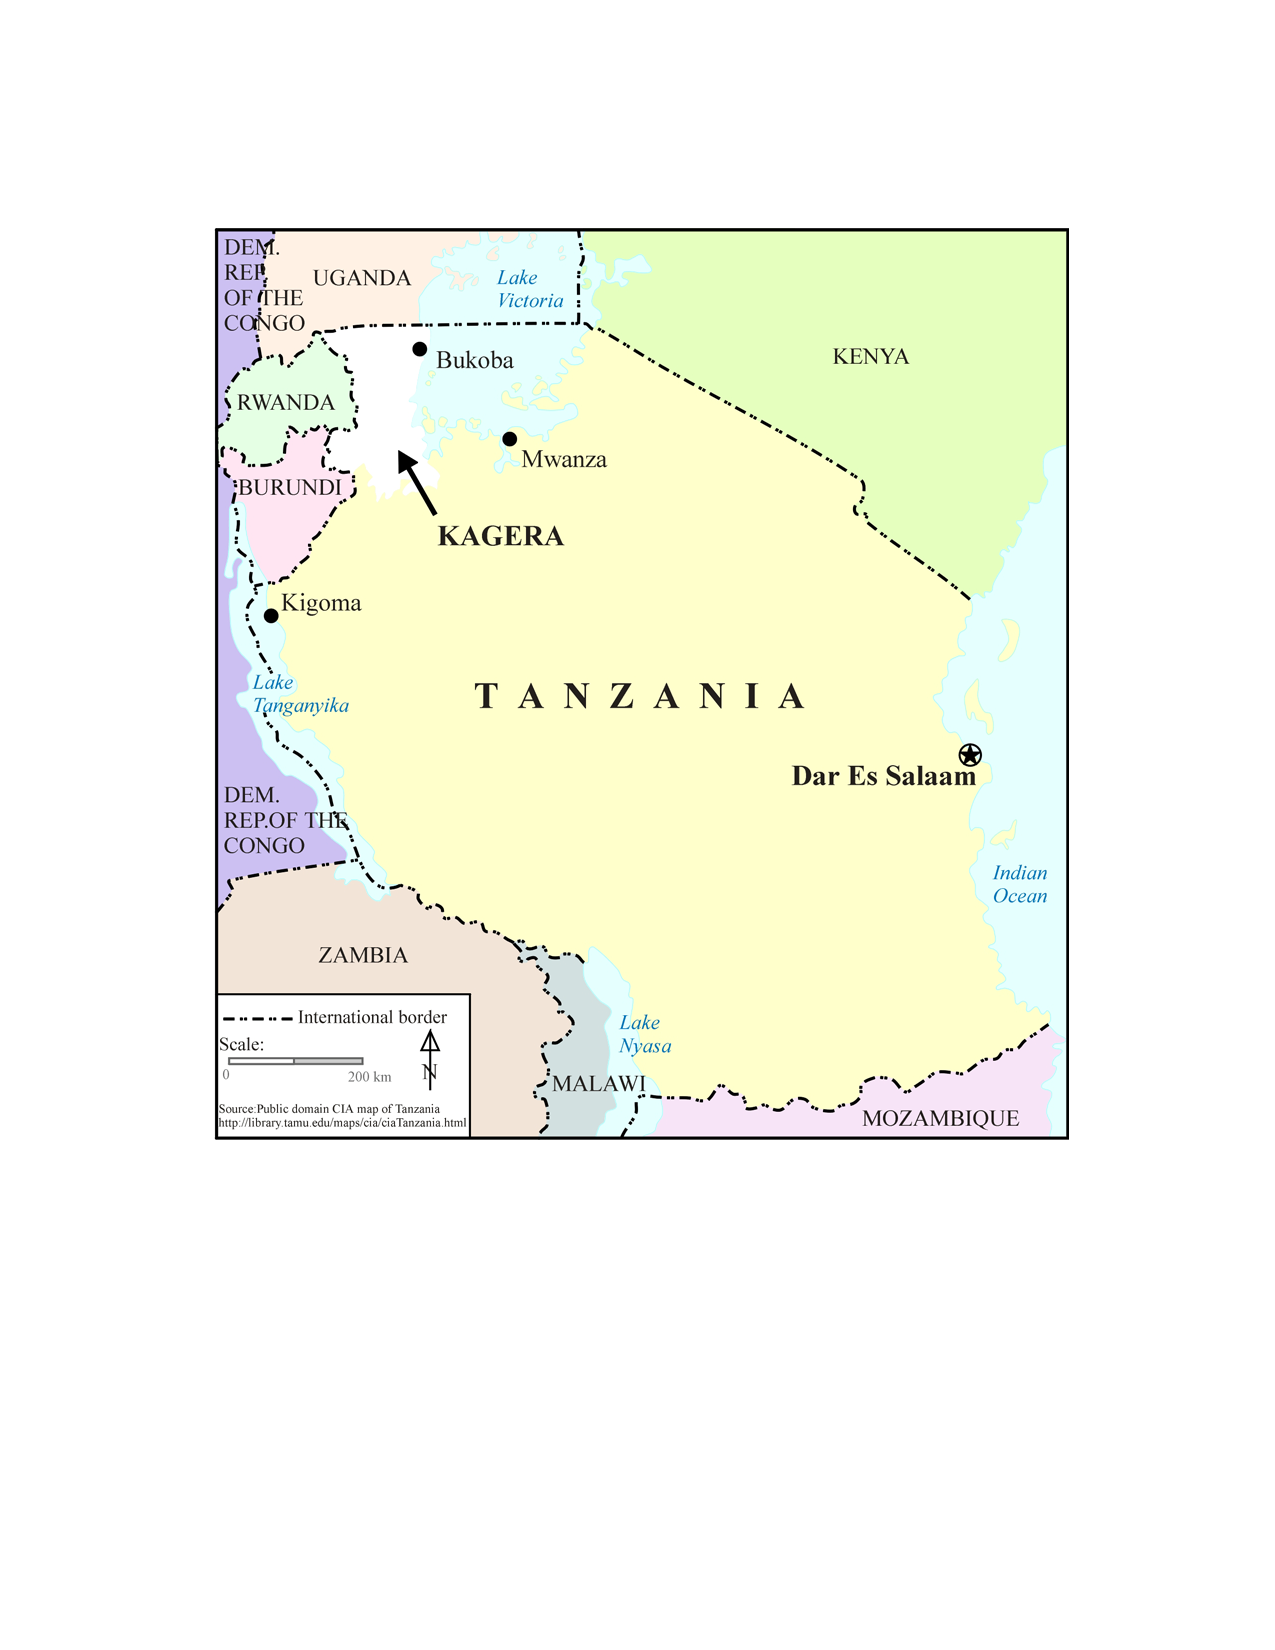
\includegraphics[width=1\textwidth]{kagera}
%     \end{column}
%     \begin{column}{.4\textwidth}
% KHDS conducted by the World Bank and the University of 
% Dar es Salaam in the Kagera region in Tanzania
% 
% \bigskip
% 
% 800 households in six districts of Kagera (Northwestern Tanzania)
%     \end{column}
%   \end{columns}
% \end{frame}


\begin{frame}{Kagera Health and Development Survey}

800 households in six districts of Kagera (Northwestern Tanzania)

\bigskip

Panel structure:
\begin{itemize}
\item Four rounds from 1991-1994 
\item Average interval between rounds 6-7 months 
\end{itemize}

\bigskip
\visible<2>{
General description:
\begin{itemize}
\item Overwhelmingly rural and primarily engaged in agriculture
\item Households use very rudimentary technology and use of wage labor is very limited
\item We use only household that have produced crops at least once and are in all 4 rounds
\end{itemize}
}
\end{frame}


\begin{frame}{Fertility and contraceptive information}

Questions to all women about their:
\begin{itemize}
\item Pregnancy
\item Child birth
\item Number of prior births
\item Current Contraception use
\item Type of contraception used (traditional and modern)
	\begin{itemize}
	\item Traditional: abstinence and rhythm method
	\item Modern: condom, diaphragm, pill, IUD, injection, female and male sterilization
	\end{itemize}
\end{itemize}
\end{frame}

% \begin{frame}{Initial evidence of impact of shocks}
% 
% \begin{center}
% % \usebeamerfont{tablefont}
% \begin{tabular}{@{} l D{.}{.}{2.1} D{.}{.}{2.1} D{.}{.}{2.1} @{}}
% 		& \multicolumn{3}{c}{Percentages}  \\
% \toprule
% 		&  			& \mco{With} & \mco{Without} \\
% 		& \mco{All} & \mco{shock} & \mco{shock} \\ \midrule
% Any contraception &	15  &  		17  &  		14  \\
% \hs Traditional    &	9  &  		10  &  		8  \\	
% \hs Modern 		   & 6  &  		7  &  		6   \\
% Pregnant	   & 14.3  &  		10.3  &  		14.4  \\
% Childbirth     & 14.0  &  		13.8  &  		14.5  \\ 	
% \bottomrule
% \end{tabular} 
% \normalfont
% \end{center}
% 
% \bigskip
% 
% Contraception: Shock 1-6 months before
% 
% Pregnancy and childbirth: Shock 7-14 months before
% 
% \end{frame}

% \begin{frame}{Frequency of shocks faced by an individual}
% 
% \begin{center}
% % \usebeamerfont{tablefont}
% \begin{tabular}{@{} l D{.}{.}{2.1} D{.}{.}{2.1} D{.}{.}{2.1} @{}}
% \toprule
% Frequency &	\mco{Number} & \mco{Percent} \\ \midrule
% 0 &	269 &	64 \\
% 1 &	135 &	32 \\
% 2 &	15 &	4 \\ \midrule
% Total &	419 & 100 \\ 
% \bottomrule \addlinespace
% N = 831 & & \\ 
% \end{tabular} 
% \normalfont
% \end{center}
% 		
% Average shocks in the past year: 	163	(19.6\%)
% 		
% \end{frame}


% \begin{frame}{Descriptive Statistics - Outcomes}
% 
% \begin{center}
% \usebeamerfont{tablefont}
% \begin{tabular}{@{} l D{.}{.}{4.2} D{.}{.}{4.2} D{.}{.}{4.2} D{.}{.}{4.2}  @{}}
% \toprule
%                                     &\multicolumn{2}{c}{Wave 3} &\multicolumn{2}{c}{Wave 4}   \\
%                             	 & \mco{Mean} 	 & 	\mco{St Dev}	 & 	\mco{Mean} 	 & 	\mco{St Dev} \\ \midrule
% Contraceptive use (percent) & & & & \\
% \hs Either	     & 	11.5	 & 	0.32	 & 	11.8	 & 	0.32 \\
% \hs Traditional	 & 	7.3	 & 	0.26	 & 	5.7	 & 	0.23 \\
% \hs Modern	 & 	4.2	 & 	0.20	 & 	6.4	 & 	0.25 \\
% Pregnant (percent)	 & 	14.3	 & 	0.35	 & 	12.8	 & 	0.33 \\
% Child birth (percent)	 & 	19	 & 	0.39	 & 	11	 & 	0.31	 & 	  \\
% Number of observations	 & 	\mct{300}	 		 & 	\mct{299} \\
% \bottomrule
% \end{tabular} 
% \normalfont
% \end{center}
% 
% \end{frame}


\begin{frame}{Descriptive statistics - wave 1 characteristics}

\begin{center}
\usebeamerfont{tablefont}
\begin{tabular}{@{} l D{.}{.}{1.2} D{.}{.}{1.2}   @{}}
\toprule
                            	 & \mco{Mean} 	 & 	\mco{St Dev}	  \\ \midrule
Age 17-22                                              &       0.221         &       0.416\\
Age 23-27                                              &       0.173         &       0.379\\
Age 28-32                                              &       0.229         &       0.421\\
Age 33-37                                              &       0.193         &       0.395\\
Age 38-45                                              &       0.185         &       0.389\\
\addlinespace
No education                                           &       0.289         &       0.454\\
1 - 6 years of education                               &       0.273         &       0.446\\
7 plus years of education                              &       0.438         &       0.497\\
\addlinespace
Assets per capita in wave 1 (1,000,000 TZS)\tnote{a}   &       0.070         &       0.127\\
\addlinespace
Number of women                                        &                \mct{249}         \\
\bottomrule
\end{tabular} 
\normalfont
\end{center}

\end{frame}


\begin{frame}{Descriptive stats - Many crop losses \& low contraceptive use}

\begin{center}
\usebeamerfont{tablefont}
\begin{tabular}{@{} l D{.}{.}{2.3} D{.}{.}{2.3} D{.}{.}{2.3} D{.}{.}{2.3} D{.}{.}{2.3}  @{}}
\toprule
                                  & \multicolumn{4}{c}{Wave} & \mco{Total} \\ \cmidrule(lr){2-5}
                                  &\multicolumn{1}{c}{1} &\multicolumn{1}{c}{2}   &\multicolumn{1}{c}{3} &\multicolumn{1}{c}{4} &   \\ \midrule
Crop loss --- 1-7 months (200+ TZS)                    &      0.69  &      0.25  &      0.01  &      0.03  &      0.25  \\
                                                       &     (0.46) &     (0.44) &     (0.09) &     (0.18) &     (0.43) \\
\addlinespace
Currently pregnant                                     &        0.16&        0.22&        0.15&        0.14&        0.17\\
                                                       &      (0.37)&      (0.42)&      (0.36)&      (0.34)&      (0.37)\\
Gave birth since last survey                           &           .&        0.16&        0.21&        0.11&        0.16\\
                                                       &         (.)&      (0.36)&      (0.41)&      (0.32)&      (0.37)\\
\addlinespace
Contraceptive use                                      &        0.14&        0.09&        0.08&        0.09&        0.10\\
                                                       &      (0.34)&      (0.28)&      (0.28)&      (0.29)&      (0.30)\\
Contraceptive use --- Traditional                      &        0.11&        0.06&        0.06&        0.04&        0.07\\
                                                       &      (0.32)&      (0.23)&      (0.25)&      (0.21)&      (0.25)\\
Contraceptive use --- Modern                           &        0.04&        0.04&        0.02&        0.05&        0.04\\
                                                       &      (0.19)&      (0.19)&      (0.15)&      (0.22)&      (0.19)\\
\bottomrule
\end{tabular} 
\normalfont
\end{center}

\end{frame}


%-------------------------------------------------------------


\section{Empirical Strategy}
\subsection{}

% \begin{frame}{Woman fixed effects model - LPM}
% 
% Dichotomous outcomes:
% \begin{itemize}
% \item Contraceptive use
% \item Pregnancy
% \item childbirth
% \end{itemize}
% 
% \bigskip
% Main explanatory variable:
% \begin{itemize}
% % Crop loss (1,000 TZS)
% \item Crop loss $\geq$ 200 TZS
% \end{itemize}
% 
% 
% \end{frame}
% 

\begin{frame}{Estimated equation - woman fixed effects LPM}

\begin{equation*}
Y_{i,t} 
=  \beta_1 croploss_{i,t}  
% +  \beta_2 croploss_{i,t} \times asset_{i,1}
+ survey_{i,t}'\mathbf{\alpha} 
+ \mu_i 
+ \varepsilon_{i,t} 
\end{equation*}


% \begin{align*}
% Y_{i,t} &=  \beta_1 croploss_{i,t}  +  \beta_2 croploss_{i,t} \times asset_{i,1} \\
% &+ survey_{i,t} \alpha + \mu_i + \varepsilon_{i,t} 
% \end{align*}

% \begin{align*}
% Y_{i,t} &=  \beta_1 Croploss_{i,t}  +  \beta_2 Croploss_{i,t} \times Asset_{i,t-2} \\
% &+ \beta_3  Croploss_{i,t-1}  +  \beta_4 Croploss_{i,t-1} \times Asset_{i,t-2}  \\
% &+ \boldsymbol{X_{i,t} \alpha} + \mu_i + \varepsilon_{i,t} 
% \end{align*}


$Y_{i,t}$:  contraception, pregnancy, or child birth - all dichotomous 


\bigskip

Main explanatory variable: Crop loss $\geq$ 200 TZS

\bigskip

% Assets are measured per capita in 10,000 TZS in wave 1
% 
% \bigskip

% $\boldsymbol{X_{i,t}}$: Number of births, number of household members, assets at $t-2$ in 1,000 TZS
% $\boldsymbol{X_{i,t}}$: Assets at $t-2$ in 1,000 TZS
$survey_{i,t}$: Survey dummies


\bigskip
 
$\mu_i$: time-invariant individual specific characteristic



\bigskip
Married/partnered women up to 45 old, who are observed in all 4 surveys


\end{frame}


% \begin{frame}{When do we observe what?}
% 
% \vspace{-20pt}
% 
%  \begin{center}
% \begin{tikzpicture}
% %draw horizontal line
% \draw (0,0) -- (9,0);
% % \draw[decorate,decoration={snake,pre length=5mm, post length=5mm}] (2,0) -- (4,0);
% %\draw (4,0) -- (5,0);
% % \draw[decorate,decoration={snake,pre length=5mm, post length=5mm}] (5,0) -- (7,0);
% 
% %draw vertical lines
% \foreach \x in {0,3,6,9}
% \draw (\x cm,3pt) -- (\x cm,-3pt);
% 
% %draw nodes - original version
% % \draw (0,0) node[below=3pt] {\small{Wave 1}} node[above=3pt] {$ $};
% % \draw (3,0) node[below=3pt] {\small{Wave 2}} node[above=3pt] {Assets$_{t-2}$};
% % \draw (4.5,0) node[below=20pt] {Croploss$_{t-1}$};
% % \draw (6,0) node[below=3pt] {\small{Wave 3}} node[above=3pt] {Assets$_{t-1}$};
% % \draw (7.5,0) node[below=20pt] {Croploss$_{t}$} node[above=54pt] {Birth$_t$};
% % \draw (9,0) node[below=3pt] {\small{Wave 4}} node[above=3pt] {Assets$_{t}$} node[above=37pt] {Contraceptive$_t$} node[above=20pt] {Pregnancy$_t$} ;
% 
% 
% % Waves
% \draw (0,0) node[below=3pt] {\small{Wave 1}} ;
% \draw (3,0) node[below=3pt] {\small{Wave 2}} ;
% \draw (6,0) node[below=3pt] {\small{Wave 3}} ;
% \draw (9,0) node[below=3pt] {\small{Wave 4}} ;
% 
% 
% % Period 3 
% \visible<2>{
% \draw (0,0) node[above=3pt] {Assets$_1$};
% \draw (1.5,0) node[below=20pt] {Croploss$_{2}$};
% \draw (4.5,0) node[below=20pt] {Croploss$_{3}$} node[above=54pt] {Birth$_3$} node[above=100pt] {\LARGE Wave 3};
% \draw (6,0) node[above=37pt] {Contraceptive$_3$} node[above=20pt] {Pregnancy$_3$};
% }
% 
% % Period 4
% \visible<3>{
% \draw (0,0) node[above=3pt] {$ $};
% \draw (3,0) node[above=3pt] {Assets$_{2}$};
% \draw (4.5,0) node[below=20pt] {Croploss$_{3}$} node[above=100pt] {\LARGE Wave 4};
% \draw (7.5,0) node[below=20pt] {Croploss$_{4}$} node[above=54pt] {Birth$_4$};
% \draw (9,0) node[above=37pt] {Contraceptive$_4$} node[above=20pt] {Pregnancy$_4$} ;
% }
% 
% \end{tikzpicture}
%  \end{center}
% 
% \end{frame}


%-------------------------------------------------------------


\section{Results}

\subsection{}

\begin{frame}{Shocks decreases pregnancies and births}

\begin{center}
\usebeamerfont{tablefont}
\begin{tabular}{@{} l D{.}{.}{2.6} D{.}{.}{2.6} D{.}{.}{2.6} D{.}{.}{2.6}  @{}}
\toprule
                                                       &\multicolumn{2}{c}{}&\multicolumn{2}{c}{Childbirth since}\\
                                                       &\multicolumn{2}{c}{Currently Pregnant}&\multicolumn{2}{c}{last survey}\\ \cmidrule(lr){2-3} \cmidrule(lr){4-5}
                                                       & \mco{OLS}           & \mco{Fixed Effects} & \mco{OLS}           & \mco{Fixed Effects} \\ \midrule
Crop loss --- 1-7 months     &      -0.064^{*}     &      -0.103^{**}    &                     &                     \\ 
\hs (200 TZS or above)       &      (0.037)        &      (0.043)        &                     &                     \\ 
Crop loss --- 7-14 months    &                     &                     &      -0.115^{***}   &      -0.175^{***}   \\ 
\hs (200 TZS or above)       &                     &                     &      (0.038)        &      (0.049)        \\ 
\addlinespace
Wave dummies                 &    \mco{Yes}        &    \mco{Yes}        &    \mco{Yes}        &    \mco{Yes}        \\
Community fixed effects      &    \mco{No}         &    \mco{No}         &    \mco{No}         &    \mco{No}         \\
Woman fixed effects          &    \mco{No}         &    \mco{Yes}        &    \mco{No}         &    \mco{Yes}        \\
Observations                 &    \mco{996}        &    \mco{996}        &    \mco{747}        &    \mco{747}        \\ 
Number of women              &    \mco{249}        &    \mco{249}        &    \mco{249}        &    \mco{249}        \\ 
\bottomrule    
\end{tabular} 
\normalfont
\end{center}

\end{frame}



\begin{frame}{Shocks also increases contraception use}

\begin{center}
\usebeamerfont{tablefont}
\begin{tabular}{@{} l D{.}{.}{2.6} D{.}{.}{2.6}  @{}}
\toprule
                                                       & \mco{OLS}           & \mco{Fixed Effects} \\ \midrule 
                                                       &\multicolumn{2}{c}{Any contraception}  \\ \cmidrule(lr){2-3}
Crop loss - 1-7 months                                 &       0.059\sym{**} &       0.075\sym{***}\\
\hs  (200 TZS or above)                                &     (0.025)         &     (0.029)         \\
\addlinespace 
                                                       &\multicolumn{2}{c}{Traditional contraception}  \\ \cmidrule(lr){2-3}
Crop loss - 1-7 months                                 &       0.056\sym{**} &       0.062\sym{**} \\
\hs  (200 TZS or above)                                &     (0.022)         &     (0.025)         \\
\addlinespace 
                                                       &\multicolumn{2}{c}{Modern contraception}  \\ \cmidrule(lr){2-3}
Crop loss - 1-7 months                                 &       0.008         &       0.020         \\
\hs  (200 TZS or above)                                &     (0.012)         &     (0.015)         \\
\addlinespace                                                        
Wave dummies                                           &    \mco{Yes}        &    \mco{Yes}        \\
Woman fixed effects                                    &    \mco{No}         &    \mco{Yes}        \\
Observations                                           &    \mco{996}        &    \mco{996}        \\
Number of women                                        &    \mco{249}        &    \mco{249}        \\
\bottomrule
\end{tabular} 
\normalfont
\end{center}

 
\end{frame}




%-------------------------------------------------------------
% 
% \subsection{Assets and Education effects}
% 
% \begin{frame}{Limited effects of assets}
% 
% 
% \begin{center}
% \usebeamerfont{tablefont}
% \begin{tabular}{@{} l D{.}{.}{2.6} D{.}{.}{2.6}  D{.}{.}{2.6}   @{}}
% \toprule
%                                                        & \mco{Pregnant}      &\mco{Childbirth}     &\mco{Contraceptives}            \\ \midrule
% Crop loss - 1-7 months                                 &      -0.095\sym{**} &                     &       0.093\sym{**} \\
% \hs  (200 TZS or above)                                &     (0.045)         &                     &     (0.037)         \\
% Crop loss - 1-7 months                                 &       0.000         &                     &      -0.003         \\
% \hs \X initial assets (10,000 TZS)                     &     (0.001)         &                     &     (0.003)         \\
% Crop loss - 7-14 months                                &                     &      -0.164\sym{***}&                     \\
% \hs  (200 TZS or above)                                &                     &     (0.053)         &                     \\
% Crop loss - 7-14 months                                &                     &       0.001         &                     \\
% \hs \X initial assets (10,000 TZS)                     &                     &     (0.002)         &                     \\
% \addlinespace 
% Wave dummies                                           &    \mco{Yes}        &    \mco{Yes}        &    \mco{Yes}        \\
% Woman fixed effects                                    &    \mco{Yes}        &    \mco{Yes}        &    \mco{Yes}        \\
% Observations                                           &    \mco{988}        &    \mco{741}        &    \mco{988}        \\
% Number of women                                        &    \mco{247}        &    \mco{247}        &    \mco{247}        \\
% \bottomrule
% \end{tabular} 
% \normalfont
% \end{center}
% \end{frame}
% 
% 
% \end{frame}
% 
% 
% \begin{frame}{Slightly larger effect for better-educated women}
% 
% \begin{center}
% \usebeamerfont{tablefont}
% \begin{tabular}{@{} l D{.}{.}{2.5} D{.}{.}{2.5}  D{.}{.}{2.5} D{.}{.}{2.5} D{.}{.}{2.5}  @{}}
% \toprule
%                                                        & \mco{}              &\mco{}               &\multicolumn{3}{c}{Contraceptive Use}\\ \cmidrule(lr){4-6}
%                                                        & \mco{Pregnant}      &\mco{Childbirth}     &\mco{Any}            &\mco{Traditional}    & \mco{Modern}        \\ \midrule
% Crop loss                                              &      -0.069         &                     &       0.080         &       0.041         &       0.032         \\
% \hs \X no education                                    &     (0.062)         &                     &     (0.051)         &     (0.041)         &     (0.029)         \\
% Crop loss                                              &      -0.006         &                     &       0.019         &       0.036         &      -0.033         \\
% \hs \X 1-6 years                                       &     (0.063)         &                     &     (0.051)         &     (0.040)         &     (0.031)         \\
% Crop loss                                              &      -0.167\sym{***}&                     &       0.098\sym{**} &       0.073\sym{*}  &       0.009         \\
% \hs \X 7+     years                                    &     (0.050)         &                     &     (0.043)         &     (0.039)         &     (0.018)         \\
% Crop loss (7-14 months)                                &                     &      -0.165\sym{**} &                     &                     &                     \\
% \hs \X no education                                    &                     &     (0.064)         &                     &                     &                     \\
% Crop loss (7-14 months)                                &                     &      -0.115         &                     &                     &                     \\
% \hs \X 1-6 years                                       &                     &     (0.072)         &                     &                     &                     \\
% Crop loss (7-14 months)                                &                     &      -0.185\sym{***}&                     &                     &                     \\
% \hs \X 7+ years                                        &                     &     (0.062)         &                     &                     &                     \\
% \addlinespace 
% Wave dummies                                           &    \mco{Yes}        &    \mco{Yes}        &    \mco{Yes}        &    \mco{Yes}        &    \mco{Yes}        \\
% Woman fixed effects                                    &    \mco{Yes}        &    \mco{Yes}        &    \mco{Yes}        &    \mco{Yes}        &    \mco{Yes}        \\
% Observations                                           &    \mco{988}        &    \mco{741}        &    \mco{988}        &    \mco{988}        &    \mco{988}        \\
% Number of women                                        &    \mco{247}        &    \mco{247}        &    \mco{247}        &    \mco{247}        &    \mco{247}        \\
% \bottomrule
% \end{tabular} 
% \normalfont
% \end{center}
% \end{frame}
% 
% \end{frame}
% 
% 




%-------------------------------------------------------------

\section{Robustness}

\subsection{What Explains the Effect?}


\begin{frame}{Shocks worsen health but not significantly}

\begin{center}
\usebeamerfont{tablefont}
\begin{tabular}{@{} l D{.}{.}{2.6} D{.}{.}{2.6}  @{}}
\toprule
                                                       & \mct{Respondent} \\
													   & \mco{BMI}           &  \mco{Illness}  	       \\ \midrule
Crop loss --- 1-7 months (200 TZS or above)            &      -0.033         &       0.022         \\
                                                       &     (0.166)         &     (0.050)         \\
Pregnant                                               &       0.831\sym{***}&                     \\
                                                       &     (0.128)         &                     \\
\addlinespace 
Wave dummies                                           &    \mco{Yes}        &    \mco{Yes}        \\
Woman fixed effects                                    &    \mco{Yes}        &    \mco{Yes}        \\
Observations                                           &    \mco{971}        &    \mco{996}        \\ 
Number of women                                        &    \mco{249}        &    \mco{249}        \\ 
\bottomrule
\end{tabular} 
\normalfont
\end{center}
 
\end{frame}



\begin{frame}{No effect on presence of partner}

\begin{center}
\usebeamerfont{tablefont}
\begin{tabular}{@{} l D{.}{.}{2.6} D{.}{.}{2.6}  @{}}
\toprule
                                                       &\mco{Absence/migration}&\mco{Dissolution of}\\
                                                       &\mco{of partner}     &\mco{ of marriage}\\ \midrule
Crop loss --- 1-7 months (200 TZS or above)            &       0.011         &      -0.004         \\
                                                       &     (0.011)         &     (0.010)         \\
\addlinespace 
Wave dummies                                           &    \mco{Yes}        &    \mco{Yes}        \\
Woman fixed effects                                    &    \mco{Yes}        &    \mco{Yes}        \\
Observations                                           &    \mco{996}        &    \mco{1329}        \\ 
Number of women                                        &    \mco{249}        &    \mco{571}        \\ 
\bottomrule
\end{tabular} 
\normalfont
\end{center}

And we use only married/partnered women
 
\end{frame}

\begin{frame}{Do contraceptive use reduce fertility?}

\begin{center}
\usebeamerfont{tablefont}
\begin{tabular}{@{} l  D{.}{.}{2.6} D{.}{.}{2.6} D{.}{.}{2.6}  @{}}
\toprule
                                                       & \multicolumn{3}{c}{Currently Pregnant} \\ \cmidrule(lr){2-4}
                                                       &\mco{Any}            & \mco{Traditional}   & \mco{Modern}        \\ \midrule
Contraceptives (7 months)                              &       0.173\sym{**} &       0.169\sym{**} &       0.163         \\
                                                       &     (0.068)         &     (0.071)         &     (0.131)         \\
Crop loss (7-14 months)                                &      -0.285\sym{**} &      -0.260\sym{**} &      -0.333\sym{*}  \\
\hs \X Contraceptives (7 months)                       &     (0.113)         &     (0.118)         &     (0.197)         \\
Crop loss --- 7-14 months (200 TZS or above)           &       0.049         &       0.041         &       0.031         \\
                                                       &     (0.050)         &     (0.049)         &     (0.048)         \\
\addlinespace 
Wave dummies                                           &    \mco{Yes}        &    \mco{Yes}        &    \mco{Yes}        \\
Woman fixed effects                                    &    \mco{Yes}        &    \mco{Yes}        &    \mco{Yes}        \\
Observations                                           &    \mco{747}        &    \mco{747}        &    \mco{747}        \\ 
Number of women                                        &    \mco{249}        &    \mco{249}        &    \mco{249}        \\ 
\bottomrule
\end{tabular} 
\normalfont
\end{center}


\end{frame}


% \begin{frame}{Other consistency checks}
% 
% Previous period contraceptive use does not predict current period shock.
% 
% \bigskip
% 
% Previous period crop loss does not predict current period crop loss.
% 
% \bigskip
% 
% Results do not change when controlling for proportion of shocks occurring in the village
% 
% \bigskip
% 
% Women do work more hours following crop loss.
% 
% 
% \end{frame}



%-------------------------------------------------------------

\section{Conclusion}

\subsection{Conclusion}

\begin{frame}{Summary}

Very poor area with low contraceptive use

\bigskip
Significant changes in timing of fertility in response to shocks
\begin{itemize}
\item Lower likelihood of pregnancy and birth
\item Main effect on traditional contraceptives
\end{itemize}

% \bigskip
% Impact significantly larger for poorer households

% \bigskip
% 
% Similar results if using education instead of assets

% \bigskip
% 
% Effect appear to be concentrated among the younger women (less than mid-30s)
% 
\end{frame}

\begin{frame}{Conclusion}


Conscious decision to postpone fertility because of shocks

\bigskip
Effect on final fertility unclear

\bigskip
Easier/better access to contraceptives could improve ability to postpone births and 
improve child health

\bigskip
Better family planning access unlikely to change overall fertility substantially 
(people already making fertility decisions)

\end{frame}

% \begin{frame}
% 
% \begin{center}
% \Huge{Thank you!}
% \end{center}
% 
% \end{frame}



%-------------------------------------------------------------

\end{document}
